\chapter{Identification, authentication, and authorisation}
\lecture{4}{29/10}

Access control is about restricting access to resources within a system. 

We refer to a \textbf{subject} as an active entity within a system (a person, a script, etc.). 
A \textbf{principal} is an entity that can be granted access (this has a unique identifier, such as a username). 

A subject will \emph{identify} itself to a system as a principal.
The system will \emph{verify} the identity of the user (password, biometrics, etc.).
The system will then check that the principal has the permissions to access an object. 

\begin{table}
    \centering
    \caption{Top 20 most popular passwords (2018).}
    \label{tab:pop-passwords}
    \begin{tabular}{rp{1.7cm}rp{1.7cm}rp{1.7cm}rp{1.7cm}}
        \toprule
        1 & 123456 & 6 & 111111 & 11 & princess & 16 & football \\
        2 & Password & 7 & 1234567 & 12 & admin & 17 & 123123 \\
        3 & 123456789 & 8 & sunshine & 13 & welcome & 18 & monkey \\
        4 & 12345678 & 9 & qwerty & 14 & 666666 & 19 & 654321 \\
        5 & 12345 & 10 & iloveyou & 15 & abc123 & 20 & \verb !@#$%^&Y* \\
        \bottomrule
    \end{tabular}
\end{table}

Table \ref{tab:pop-passwords} illustrates a major issue with passwords. Common security guidelines are
\begin{enumerate}
    \item adopt long passwords;
    \item avoid easy to guess passwords;
    \item use alphanumeric;
    \item do not write down passwords; and
    \item avoid using the same password for multiple services.
\end{enumerate}

It is easy that expecting a subject to remember a separate password that is long and cannot be written down anywhere is not a reasonable task. A solution here is to store passwords is password-protected password agents (such as LastPass, DashLane, etc.).

\begin{definition}[Authentication key]
    An \textbf{authentication key} are similar to passwords but are RSA-keys. Subjects create a private and a public key (public to encrypt and priate to decrypt) and they share the public key with services. 
\end{definition}

Authentication are beneficial as a public key leak is inconsequential. Additionally, compromised device access can be revoked. However, authentiation keys have their weakness if there is a compromised client. The solution to this are physical security keys, such as: static password token (not recommended), asynchoronous tokens (one-time passwords), and challenge-response tokens.

\begin{definition}[Biometrics]
    \textbf{Biometrics} is the technical term for body measurements and calculations.
\end{definition}

\begin{example}[Biometrics]
    \begin{enumerate}
        \item Face recognition;
        \item fingerprints;
        \item iris recognition;
        \item gait recognition (how you walk); and
        \item DNA matching.
    \end{enumerate}
\end{example}

Biometrics have the advantage of being able to guarantee that accesses a certain facility; they cannot later deny it. 
Biometrics have a reputation for having false-positives and false-negatives. 
Figure \ref{fig:false-match-rate} shows false match rate plotted on the false non-match rate for different biometrics. 
Technologies with a low false non-match rate but a high false match rate are good for suspect recognition from CCTV.
Alternatively, technologies with a low false match rate but a high false non-match rate are good for automatic border control. 

\begin{figure}
    \centering
    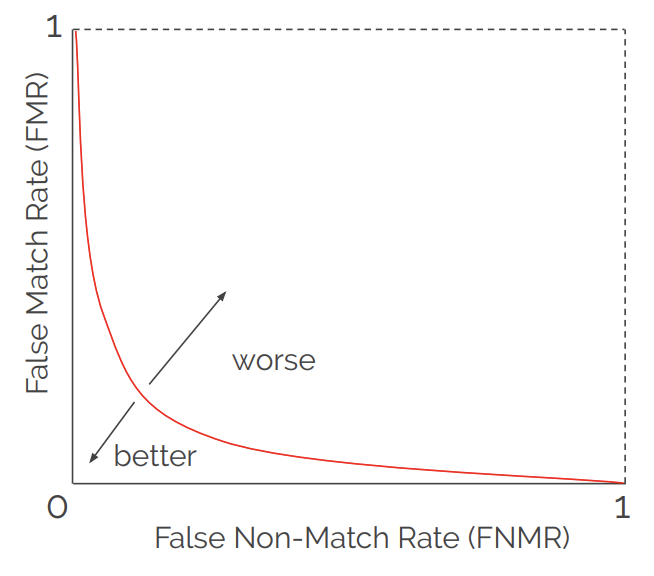
\includegraphics[width=0.6\linewidth]{images/false-match-rate.png}
    \caption{Receiver operating characteristic (ROC) curve.}
    \label{fig:false-match-rate}
\end{figure}

\begin{definition}[Multi-factor authentication]
    \textbf{Multi-factor authentication} is an authentication method in which a computer grants access only after two or more pieces of evidence (factors) are provided.
\end{definition}

We can easily define \textbf{two-factor authentication} as a subset of multi-factor authentication where only \emph{two} factors are needed.

\begin{example}[Bitcoin]
    Bitcoin uses a public and private key authentication factor. Each transaction output has an associated script controllign permissions. 
\end{example}

\begin{definition}[Zero-knowledge password proof]
    \textbf{Zero-knowledge password proof} is a method in which one party can verify to another that it knows the value of the password, without revealing anything other than the fact that it knows the password.
\end{definition}

\begin{example}[Challenge-response authentication]
    The most common approach is \emph{challenge-response authentication}, as follows.
    \begin{enumerate}
        \item The server generates a unique challenge value: nonce.
        \item The server sends nonce to the client.
        \item The client computes the response as $\operatorname{hash}(\text{nonce} + \text{password})$.
        \item The client sends response back to the server.
        \item The server compares the response with its own hash calculated with its stored password.
    \end{enumerate}
    This is a good approach, except that it is susceptible to PRNG flaws.
\end{example}

% todo EMV payments?
